\section{Exercises}

These exercises are taken from the course workbook\cite{exerciseBook}. In the following sections you can see how we approached the exercises.

\subsection{Availability}

\subsubsection{Collection and analysis}

\descriptionproblem
Consider the system in Figure~\ref{fig: exercises - collection and analysis system}. Assume that the participating components offer the following availability:
\begin{itemize}
    \item \texttt{DataCollector}: 99\%
    \item \texttt{MessageQueue}: 99.99\%
    \item \texttt{DataAnalyzer}: 99.5\%
\end{itemize}

\begin{figure}[!htp]
    \centering
    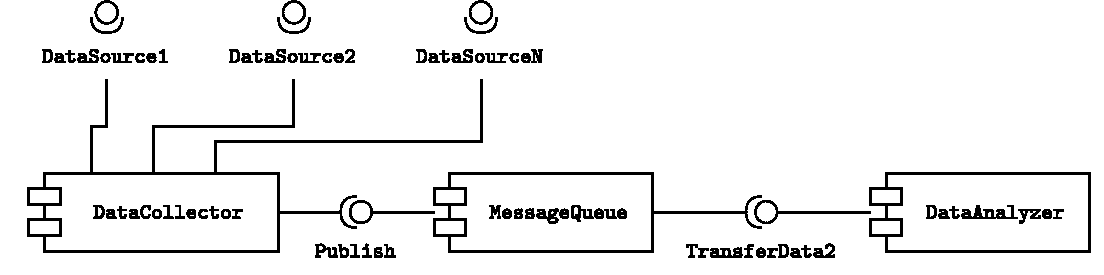
\includegraphics[width=\textwidth]{img/collection-and-analysis-1.pdf}
    \caption{Collection and analysis system.}
    \label{fig: exercises - collection and analysis system}
\end{figure}

\questionproblem
\begin{enumerate}
    \item Provide an estimate of your system's total availability (a rough estimation is acceptable without complete calculations). Assume you want to improve this total availability through replication, which component(s) would you choose to replicate? Explain your reasoning.
    
    \item How would such replication impact the way the system works and is designed?
\end{enumerate}

\solution
\textbf{\underline{Solution 1}.} We can use Equation~\ref{eq: availability in series} on page~\pageref{eq: availability in series} to estimate our system's total availability. Then, we can multiply the availability of each item in the system:
\begin{equation*}
    \begin{array}{rcl}
        \texttt{Availability} &=& \texttt{DataCollector} \times \texttt{MessageQueue} \times \texttt{DataAnalyzer} \\ [.5em]
        %
        &=& \left(99 \div 100\right) \times \left(99.99 \div 100\right) \times \left(99.5 \div 100\right) \\ [.5em]
        %
        &=& 0.99 \times 0.9999 \times 0.995 \\ [.5em]
        %
        &=& 0.984951495 \approx 0.985
    \end{array}
\end{equation*}
Now, we want to improve the system's accessibility. As the exercise suggests, we use the replication technique. Since the component to replicate is the worst, we replicate the \texttt{DataAnalyzer} (99.5\% availability).

So, how can we calculate accessibility? Well, when we replicate a component, we take advantage of the \emph{parallel} concept. Then, we use Equation~\ref{eq: availability in parallel} (page~\pageref{eq: availability in parallel}) on these components. Finally, the availability becomes:
\begin{equation*}
    \begin{array}{rcl}
        \texttt{Improved Avail.} &=& 0.99 \times 0.9999 \times \left[1 - \left(1 - 0.995\right)\times\left(1 - 0.995\right)\right] \\ [.5em]
        %
        &=& 0.989901 \times \left[1 - 0.000025\right] \\ [.5em]
        %
        &=& 0.989901 \times 0.999975 \\ [.5em]
        %
        &=& 0.989876252475 \approx 0.989 \approx 0.99
    \end{array}
\end{equation*}

\highspace
\textbf{\underline{Solution 2}.} We have improved the availability system with replication, but how are two parallel components managed? We can choose between three available tactics (page~\pageref{Replication approaches}): Hot Spare, Warm Spare, and Cold Spare (\emph{Triple Modular Redundancy} cannot be applied because there are only two parallel modules).
\begin{itemize}
    \item \emph{Hot Spare} approach: \texttt{DataCollector1} and \texttt{DataCollector2} are updated at the same time from the \texttt{MessageQueue}. One component leads, and another is always ready to take over.
    
    However, the main problem with this choice is the \emph{data duplication}. Because when the two components receive the same data, both process and return the information at the source \texttt{MessageQueue}. To manage this issue, we can code a system to avoid duplicates on the queue. 
    
    Another issue when two sources answer simultaneously is \emph{concurrency} (a race condition problem). This problem can be solved by implementing mutual exclusion mechanisms.


    \item \emph{Warm} or \emph{Cold Spare}: In the first, \texttt{DataCollector1} leads and periodically updates the \texttt{DataCollector2}. If the primary \texttt{DataCollector} fails, the second \texttt{DataCollector} takes time to update itself fully. In the second, \texttt{DataCollector2} is dormant, and it's started and updated only if required.
\end{itemize}
